\documentclass[draft]{agujournal2019}
\usepackage{url}
\usepackage{lineno}
\usepackage{longtable}

\linenumbers

\draftfalse

\journalname{JGR: Solid Earth}

\renewcommand{\thefigure}{S\arabic{figure}}
\renewcommand{\thetable}{S\arabic{table}}

\begin{document}

\title{An eight-year-long low-frequency earthquake catalog for Southern Cascadia}

\authors{Ariane Ducellier\affil{1}, Kenneth C. Creager\affil{1}}

\affiliation{1}{University of Washington}

\correspondingauthor{Ariane Ducellier}{ducela@uw.edu}

\begin{figure}[hbt!]
\noindent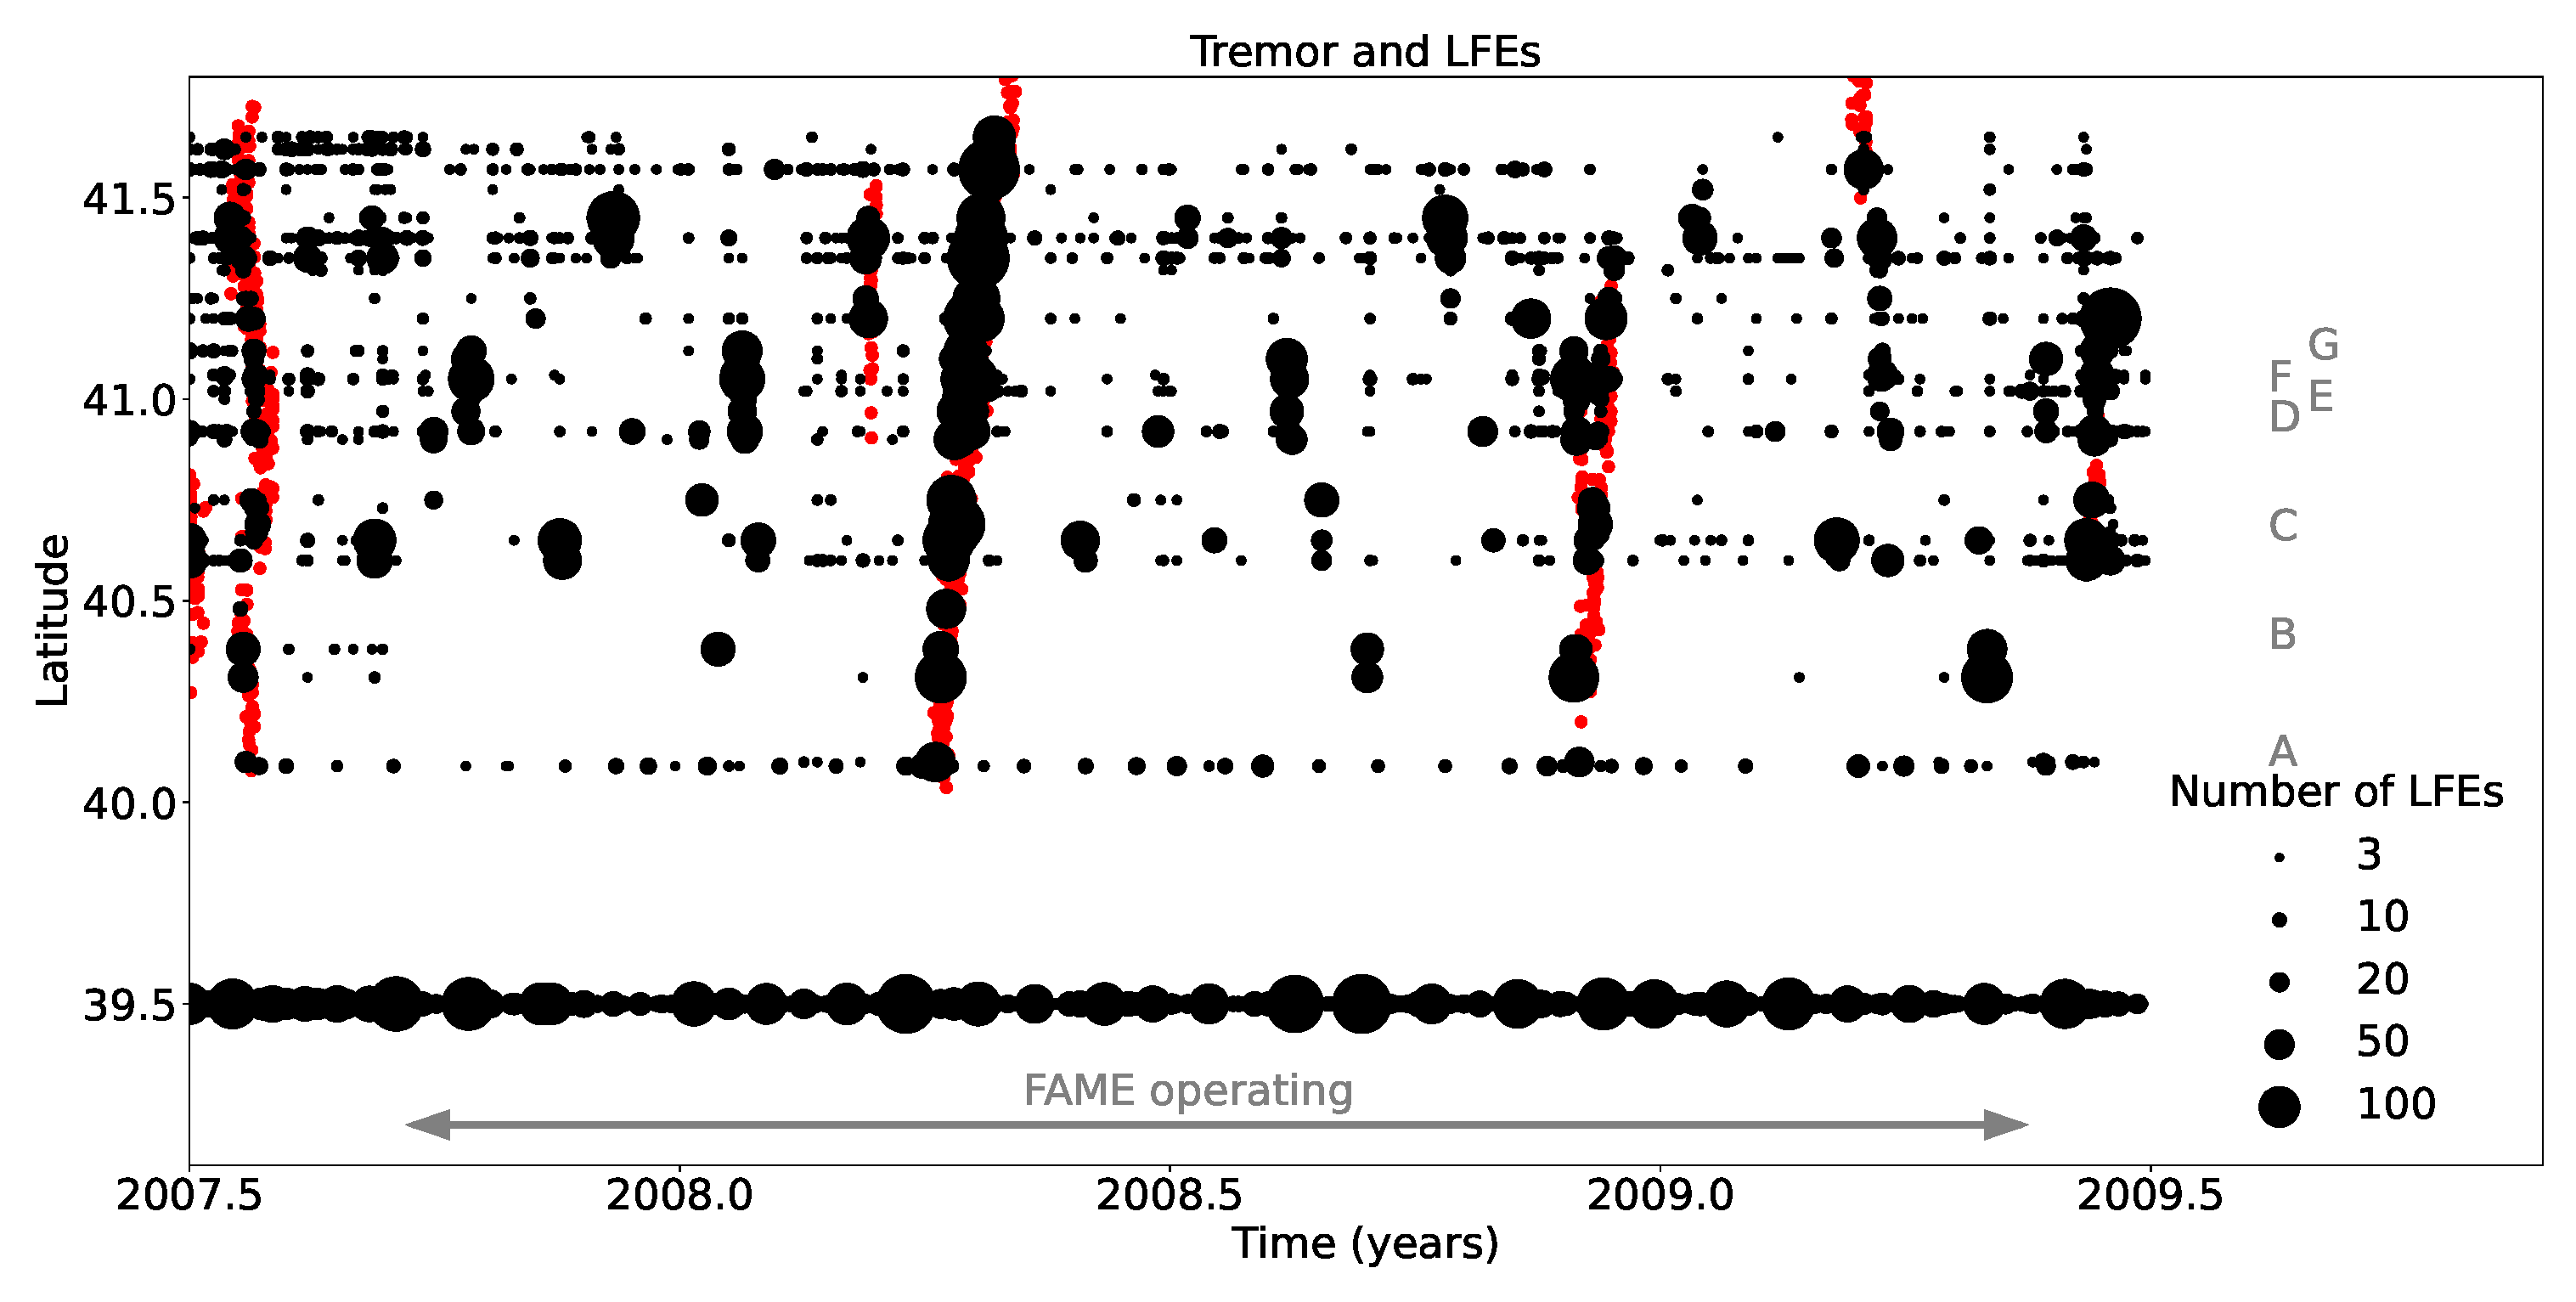
\includegraphics[width=\textwidth, trim={0cm 0cm 0cm 0cm},clip]{figures/unfiltered_FAME.eps}
\caption{Same as Figure 3 from the main text, but without filtering the LFEs. They are many false detections at the beginning and the end of the catalog because the FAME stations were not yet installed / already removed.}
\label{pngfiguresample}
\end{figure}

\begin{figure}[hbt!]
\noindent\includegraphics[width=\textwidth, trim={0cm 0cm 0cm 0cm},clip]{figures/unfiltered_perm.eps}
\caption{Same as Figure 6 from the main text, but without filtering the LFEs.}
\label{pngfiguresample}
\end{figure}

\begin{figure}[hbt!]
\noindent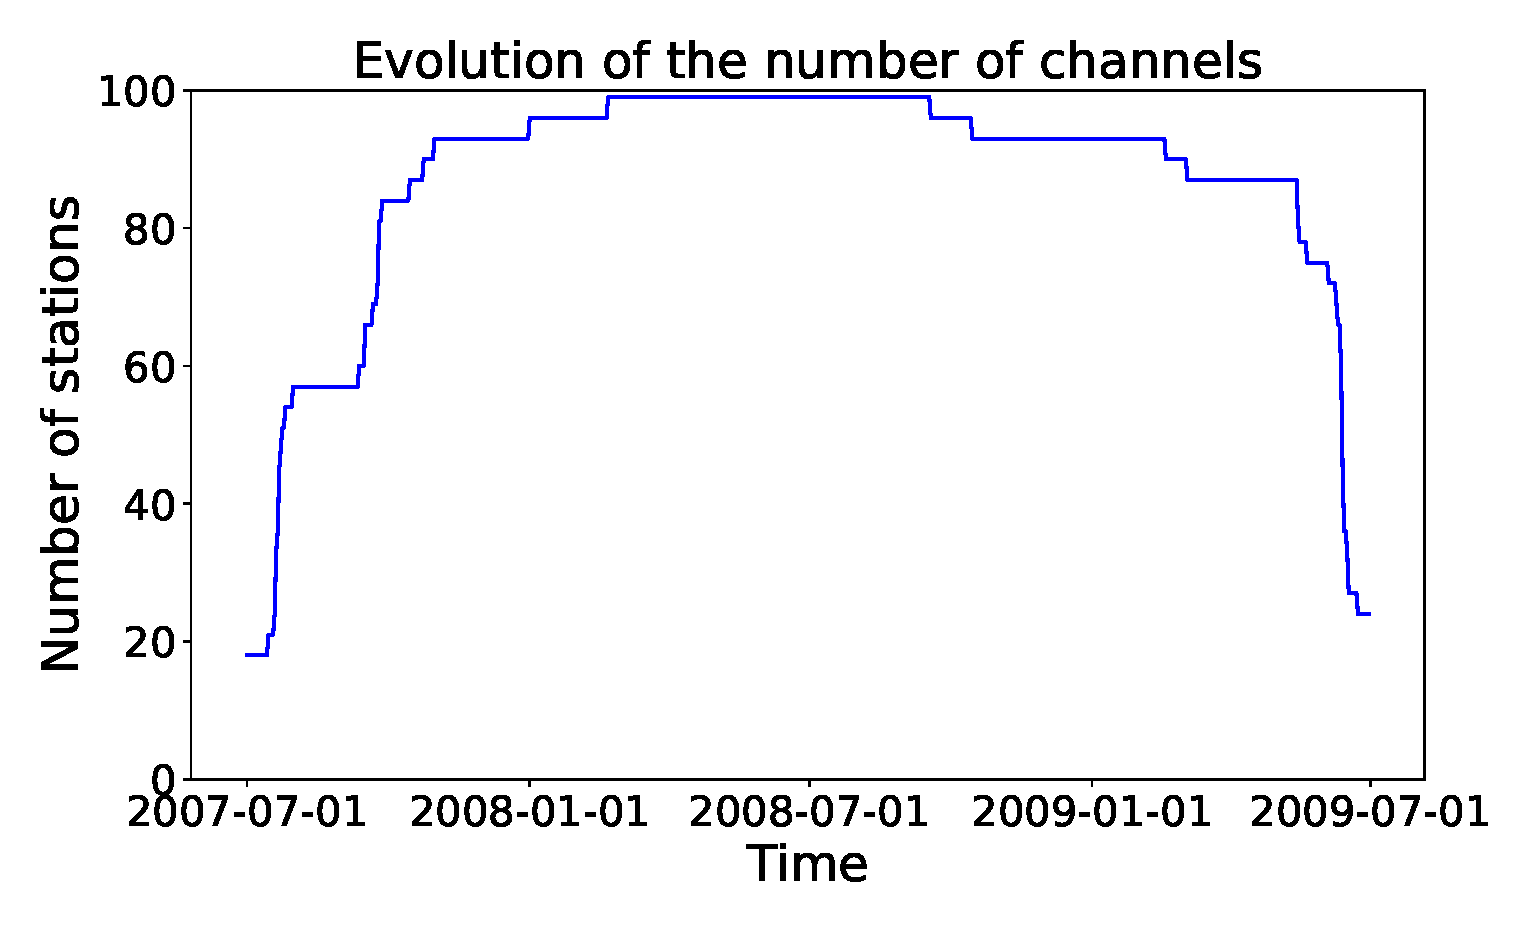
\includegraphics[width=\textwidth, trim={0cm 0cm 0cm 0cm},clip]{figures/timeline_FAME.eps}
\caption{Evolution of the number of channels available for the computation of the 2007-2009 catalog using the temporary FAME stations.}
\label{pngfiguresample}
\end{figure}

\begin{figure}[hbt!]
\noindent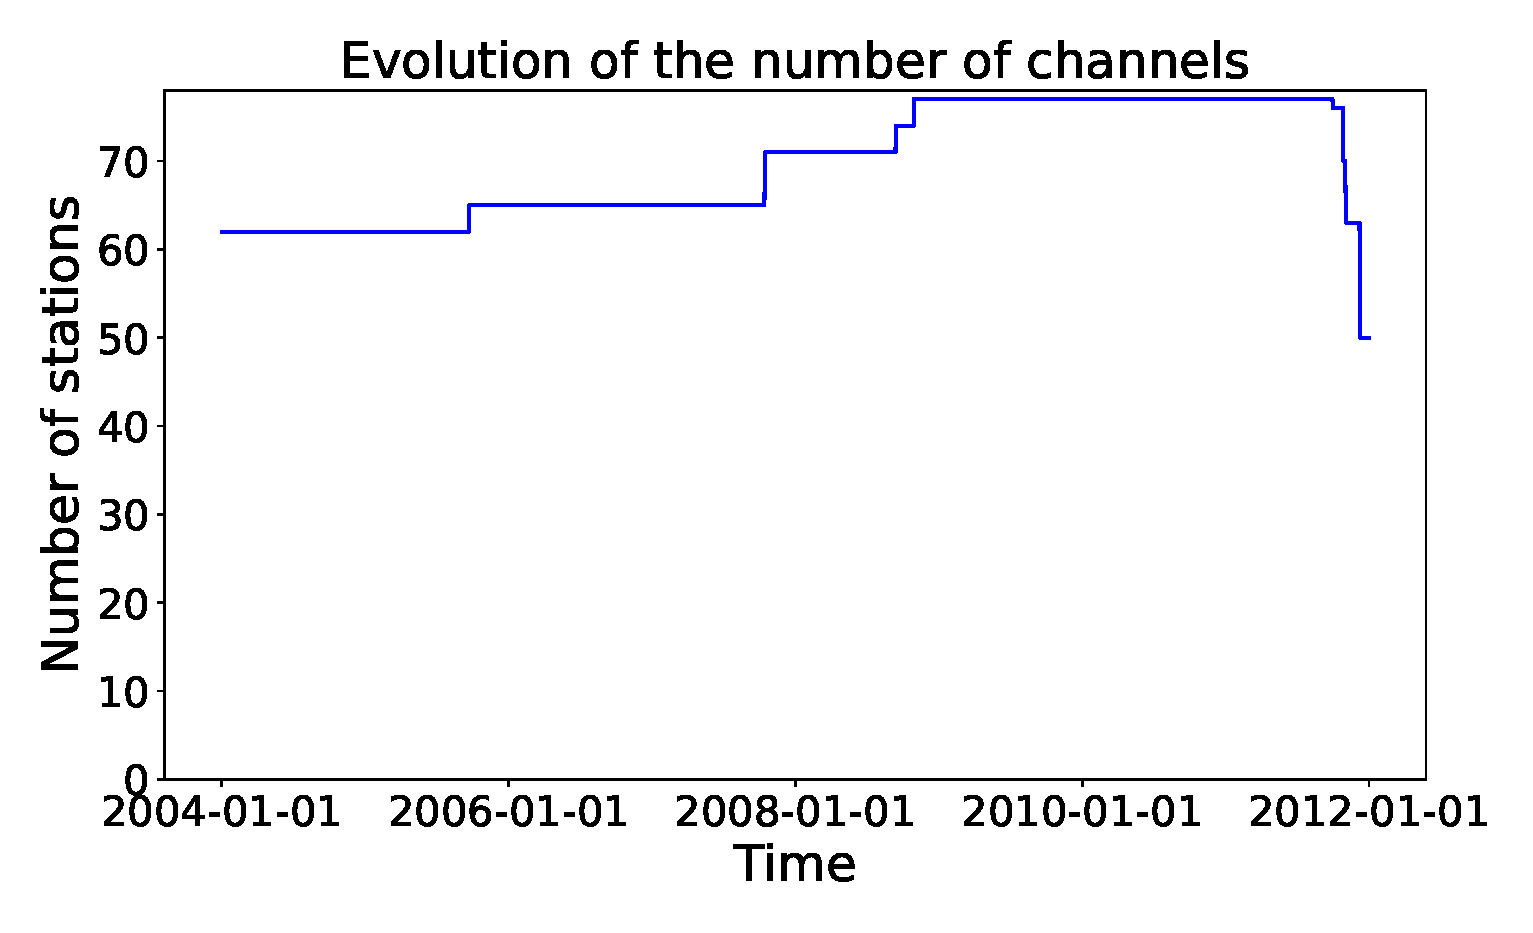
\includegraphics[width=\textwidth, trim={0cm 0cm 0cm 0cm},clip]{figures/timeline_perm.eps}
\caption{Evolution of the number of channels available for the computation of the 2004-2011 catalog using the permanent stations.}
\label{pngfiguresample}
\end{figure}

\newpage

\begin{table}[hbt!]
\caption{Temporary stations used for the 2007-2009 catalog. The data centers providing the seismic waveforms are the Incorporated Research Institutions for Seismology (IRIS) (Alan Levander, 2007), and the Northern California Earthquake Data Center (NCEDC), doi:10.7932/NCEDC.}
\centering
\footnotesize
\begin{tabular}{c c c c c c c c c}
\hline
Station & Network & Channels & Location & Data center & Latitude & Longitude & Begin time & End time \\
\hline
B039 & PB & EH1,EH2,EHZ & -- & IRIS & 41.4667 & -122.4847 & 2007-10-15 & 3000-01-01 \\
KCPB & NC & HHE,HHN,HHZ & -- & NCEDC & 39.6863 & -123.5824 & 2002-10-17 & 3000-01-01 \\
KHBB & NC & HHE,HHN,HHZ & -- & NCEDC & 40.6599 & -123.2197 & 2003-09-11 & 3000-01-01 \\
KRMB & NC & HHE,HHN,HHZ & -- & NCEDC & 41.5230 & -123.9080 & 2001-06-16 & 3000-01-01 \\
KSXB & NC & HHE,HHN,HHZ & -- & NCEDC & 41.8304 & -123.8769 & 2001-07-13 & 3000-01-01 \\
ME01 & XQ & BHE,BHN,BHZ & 01 & IRIS & 41.7752 & -123.4034 & 2007-07-31 & 2009-06-12 \\
ME02 & XQ & BHE,BHN,BHZ & 01 & IRIS & 41.6898 & -122.3372 & 2007-07-22 & 2009-05-20 \\
ME03 & XQ & BHE,BHN,BHZ & 01 & IRIS & 41.702 & -123.881 & 2007-09-27 & 2009-06-13 \\
ME04 & XQ & BHE,BHN,BHZ & 01 & IRIS & 41.355 & -123.514 & 2007-07-23 & 2009-06-12 \\
ME08 & XQ & BHE,BHN,BHZ & 01 & IRIS & 40.222 & -123.305 & 2007-07-22 & 2009-06-03 \\
ME09 & XQ & BHE,BHN,BHZ & 01 & IRIS & 41.086 & -122.726 & 2007-07-21 & 2009-05-14 \\
ME10 & XQ & BHE,BHN,BHZ & 01 & IRIS & 40.9591 & -122.4619 & 2007-10-31 & 2009-06-12 \\
ME12 & XQ & BHE,BHN,BHZ & 01 & IRIS & 40.104 & -122.498 & 2007-07-20 & 2009-06-12 \\
ME13 & XQ & BHE,BHN,BHZ & 01 & IRIS & 40.764 & -122.918 & 2007-07-22 & 2009-06-12 \\
ME16 & XQ & BHE,BHN,BHZ & 01 & IRIS & 40.577 &  -122.087 & 2007-07-20 & 2008-10-14 \\
ME24 & XQ & BHE,BHN,BHZ & 01 & IRIS & 40.359 & -122.047 & 2007-07-19 & 2009-05-15 \\
ME26 & XQ & BHE,BHN,BHZ & 01 & IRIS & 40.157 & -122.099 & 2007-07-26 & 2009-02-17 \\
ME27 & XQ & BHE,BHN,BHZ & 01 & IRIS & 40.453 & -123.155 & 2008-01-01 & 2009-06-13 \\
ME28 & XQ & BHE,BHN,BHZ & 01 & IRIS & 40.327 & -122.471 & 2007-07-20 & 2009-05-14 \\
ME29 & XQ & BHE,BHN,BHZ & 01 & IRIS & 41.142 & -123.1408 & 2007-09-21 & 2009-06-13 \\
ME30 & XQ & BHE,BHN,BHZ & 01 & IRIS & 40.843 & -123.565 & 2007-07-24 & 2009-06-22 \\
ME42 & XQ & BHE,BHN,BHZ & 01 & IRIS & 39.7145 & -123.273 & 2007-07-15 & 2009-06-16 \\
ME43 & XQ & BHE,BHN,BHZ & 01 & IRIS & 39.5703 & -123.175 & 2007-09-16 & 2009-06-16 \\
ME44 & XQ & BHE,BHN,BHZ & 01 & IRIS & 39.4928 & -123.187 & 2007-09-16 & 2009-06-15 \\
ME45 & XQ & BHE,BHN,BHZ & 01 & IRIS & 39.4666 & -122.9595 & 2007-09-12 & 2009-06-09 \\
ME46 & XQ & BHE,BHN,BHZ & 01 & IRIS & 39.196 & -122.968 & 2007-09-25 & 2009-06-11 \\
ME47 & XQ & BHE,BHN,BHZ & 01 & IRIS & 39.1124 & -122.8106 & 2007-09-25 & 2008-09-17 \\
ME49 & XQ & BHE,BHN,BHZ & 01 & IRIS & 39.8633 & -123.7194 & 2007-09-25 & 2009-06-08 \\
ME52 & XQ & BHE,BHN,BHZ & 01 & IRIS & 39.3228 & -123.2191 & 2008-02-21 & 2009-07-08 \\
ME54 & XQ & BHE,BHN,BHZ & 01 & IRIS & 39.0132 & -123.3779 & 2007-09-24 & 2009-03-03 \\
ME57 & XQ & BHE,BHN,BHZ & 01 & IRIS & 39.9118 & -122.5676 & 2007-10-24 & 2009-06-11 \\
WDC & BK & BHE,BHN,BHZ & -- & NCEDC & 40.5799 & -122.5411 &1992-09-17 & 2011-05-06 \\
YBH &  BK & BHE,BHN,BHZ & -- & NCEDC & 41.7320 & -122.7104 & 1993-07-24 & 2011-06-03 \\
\hline
\end{tabular}
\end{table}

\newpage

\begin{table}[hbt!]
\caption{Permanent stations used for the 2004-2011 catalog. The data centers providing the seismic waveforms are the Incorporated Research Institutions for Seismology (IRIS) (Alan Levander, 2007), and the Northern California Earthquake Data Center (NCEDC), doi:10.7932/NCEDC.}
\centering
\footnotesize
\begin{tabular}{c c c c c c c c c}
\hline
Station & Network & Channels & Location & Data center & Latitude & Longitude & Begin time & End time \\
\hline
B039 & PB & EH1,EH2,EHZ & -- & IRIS & 41.4667 &  -122.4847 & 2007-10-15 & 3000-01-01 \\
B040 & PB & EH1,EH2,EHZ & -- & IRIS & 41.8308 &  -122.4205 & 2007-10-16 & 3000-01-01 \\
B933 & PB & EH1,EH2,EHZ & -- & IRIS & 40.0600 &  -123.9690 & 2008-09-13 & 3000-01-01 \\
B935 & PB & EH1,EH2,EHZ & -- & IRIS & 40.4787 &  -123.5732 & 2008-10-29 & 3000-01-01 \\
GASB & BK & BHE,BHN,BHZ & -- & NCEDC & 39.65471 & -122.71595 & 2005-09-22 & 2011-06-16 \\
GASB & BK & BHE,BHN,BHZ & 0 & NCEDC & 39.65471 & -122.71595 & 2011-06-16 & 3000-01-01 \\
GBB & NC & EHZ & -- & NCEDC & 39.80127 & -122.34550 & 2000-12-06 & 3000-01-01 \\
GHM & NC & EHZ & -- & NCEDC & 39.49545 & -122.93096 & 1984-01-01 & 3000-01-01 \\
GRO & NC & EHZ & -- & NCEDC & 39.91684 & -122.67117 & 1990-12-13 & 3000-01-01 \\
GSN & NC & EHZ & -- & NCEDC & 38.94040 & -123.19245 & 1984-01-01 & 2018-12-11 \\
GTC & NC & SHZ & -- & NCEDC & 39.39944 & -123.55532 & 1996-08-01 & 2011-10-27 \\
GVV & NC & EHZ & -- & NCEDC & 39.77510 & -122.67551 & 2002-04-28 & 3000-01-01 \\
HOPS & BK & BHE,BHN,BHZ & -- & NCEDC & 38.99349 & -123.07234 & 1994-10-21 & 2010-06-16 \\
HOPS & BK & BHE,BHN,BHZ & 0 & NCEDC & 38.99349 & -123.07234 & 2010-06-16 & 3000-01-01 \\
JCC & BK & BHE,BHN,BHZ & -- & NCEDC & 40.81745 & -124.02955 & 2001-04-11 & 2010-08-19 \\
JCC & BK & BHE,BHN,BHZ & 0 & NCEDC & 40.81745 & -124.02955 & 2010-08-19 & 3000-01-01 \\
KBN & NC & SHZ & -- & NCEDC & 39.89237 & -123.19503 & 1994-11-28 & 2011-10-27 \\
KBS & NC & SHZ & -- & NCEDC & 39.91719 & -123.59561 & 2002-10-17 & 2011-10-27 \\
KCPB & NC & HHE,HHN,HHZ & -- & NCEDC & 39.68631 & -123.58242 & 2002-10-17 & 3000-01-01 \\\
KCS & NC & SHZ & -- & NCEDC & 40.53791 & -123.51394 & 1994-11-28 & 2011-11-01 \\
KFP & NC & SHZ & -- & NCEDC & 39.63889 & -123.42514 & 1994-11-28 & 2011-10-27 \\
KHBB & NC & HHE,HHN,HHZ & -- & NCEDC & 40.65990 & -123.21966 & 2003-09-11 & 3000-01-01 \\
KHMB & NC & HHE,HHN,HHZ & -- & NCEDC & 40.87475 & -123.73259 & 2002-06-13 & 3000-01-01 \\
KIP & NC & SHZ & -- & NCEDC & 39.80841 & -123.48130 & 1994-11-28 & 2011-10-27 \\
KKP & NC & SHZ & -- & NCEDC & 40.14579 & -123.46965 & 1994-11-28 & 2011-11-01 \\
KOM & NC & SHZ & -- & NCEDC & 41.27872 & -123.45315 & 1994-11-28 & 2011-11-02 \\
KPP & NC & SHZ & -- & NCEDC & 40.34579 & -123.36328 & 1994-11-28 & 2011-11-01 \\
KRK & NC & SHZ & -- & NCEDC & 39.56315 & -123.18367 & 1994-11-28 & 2011-10-27 \\
KRMB & NC & HHE,HHN,HHZ & -- & NCEDC & 41.52296 & -123.90797 & 2001-06-16 & 3000-01-01 \\
KRP & NC & HHE,HHN,HHZ & -- & NCEDC & 41.15765 & -124.02330 & 2002-06-12 & 3000-01-01 \\
KSXB & NC & HHE,HHN,HHZ & -- & NCEDC & 41.83038 & -123.87688 & 2001-07-13 & 3000-01-01 \\
KTR & NC & SHZ & -- & NCEDC & 41.90847 & -123.37755 & 1994-11-28 & 2011-11-02 \\
LAM & NC & SHZ & -- & NCEDC & 41.60987 & -122.62559 & 1994-11-28 & 2011-09-30 \\
LBF & NC & SHZ & -- & NCEDC & 41.34707 & -121.89098 & 1994-11-28 & 2011-11-03 \\
LBK & NC & SHZ & -- & NCEDC & 41.08382 & -122.66731 & 1994-11-28 & 2011-12-08 \\
LBP & NC & SHZ & -- & NCEDC & 40.31671 & -122.88193 & 1994-11-28 & 2011-12-08 \\
LDB & NC & SHZ & -- & NCEDC & 40.43105 & -121.78632 & 1994-11-28 & 2011-12-08 \\
LGB & NC & SHZ & -- & NCEDC & 41.33418 & -122.18771 & 2001-10-20 & 2011-11-03 \\
LGP & NC & SHZ & -- & NCEDC & 40.91228 & -122.82949 & 1994-11-28 & 2011-12-08 \\
LPG & NC & SHZ & -- & NCEDC & 40.14514 & -122.68788 & 1994-11-28 & 2011-12-08 \\
LRB & NC & SHZ & -- & NCEDC & 40.14323 & -122.55772 & 1994-11-28 & 2011-12-08 \\
LRR & NC & SHZ & -- & NCEDC & 40.46630 & -121.62230 & 1994-11-28 & 2011-12-08 \\
LSF & NC & SHZ & -- & NCEDC & 40.65817 & -122.52371 & 1994-11-28 & 2011-12-08 \\
LSH & NC & SHZ & -- & NCEDC & 40.79294 & -122.03943 & 2002-03-28 & 2011-12-08 \\
LSR & NC & SHZ & -- & NCEDC & 41.10696 & -122.27062 & 1994-11-28 & 2011-12-08 \\
LTC & NC & SHZ & -- & NCEDC & 40.20842 & -122.12548 & 2002-03-28 & 2011-12-08 \\
LVR & NC & SHZ & -- & NCEDC & 40.03937 & -122.67250 & 1994-11-28 & 2011-12-08 \\
LWH & NC & SHZ & -- & NCEDC & 40.64180 & -121.94857 & 1994-11-28 & 2011-12-08 \\
WDC & BK & BHE,BHN,BHZ & -- & NCEDC & 40.57988 & -122.54113 & 1992-09-17 & 2011-05-06 \\
WDC & BK & BHE,BHN,BHZ & 0 & NCEDC & 40.57988 & -122.54113 & 2011-05-06 & 3000-01-01 \\
YBH & BK & BHE,BHN,BHZ & -- & NCEDC & 41.73204 & -122.71039 & 1993-07-24 & 2011-06-03 \\
YBH & BK & BHE,BHN,BHZ & 0 & NCEDC & 41.73204 & -122.71039 & 2011-06-03 & 3000-01-01 \\
\hline
\end{tabular}
\end{table}

\newpage

\begin{table}[hbt!]
\caption{Thresholds used to clean the catalogs. An LFE is kept in the catalog if its cross-correlation value multiplied by the number of channels recording when it was detected is higher than the threshold. The threshold is missing for the families for which there were not enough permanent stations with good templates to obtain reliable LFE detections.}
\centering
\scriptsize
\begin{tabular}{c c c}
\hline
Family & Threshold 2007-2009 FAME catalog & Threshold 2004-2011 networks catalog\\
\hline
080401.05.050 & 1.4 & 1.9 \\
080405.11.042 & 2.0 & 1.6 \\
080408.08.007 & 1.7 & 1.5 \\
080408.15.023 & 2.0 & 1.3 \\
080408.08.029 & 2.3 & 1.4 \\
080408.16.026 & 1.8 & 1.4 \\
080410.01.050 & 3.5 & 1.3 \\
080410.09.032 & 3.9 & 1.4 \\
080410.12.039 & 1.9 & 1.3 \\
080410.12.040 & 5.4 & 2.3 \\
080411.04.013 & 3.4 & 1.5 \\
080411.04.023 & 3.6 & 1.5 \\
080410.13.055 & 1.9 & 1.3 \\
080412.03.029 & 2.2 & 1.0 \\
080412.11.038 & 2.2 & 1.3 \\
080412.22.047 & 3.2 & 1.5 \\
080413.13.026 & 2.2 & 1.3 \\
080412.22.040 & 3.5 & 1.6 \\
080413.07.015 & 2.0 & 1.6 \\
080413.07.023 & 1.8 & 1.4 \\
080413.16.058 & 2.2 & 0.1 \\
080413.18.013 & 2.6 & 1.2 \\
080413.20.036 & 2.1 & 1.1 \\
080414.12.016 & 2.0 & 1.2 \\
080414.12.020 & 1.5 & 1.2 \\
080414.10.058 & 1.8 & 1.2 \\
080414.18.003 & NA & NA \\
080415.11.006 & 4.6 & 1.6 \\
080415.11.008 & 3.0 & 1.8 \\
080415.24.028 & 2.5 & 1.7 \\
080416.15.003 & 2.8 & 1.7 \\
080418.03.001 & 5.0 & 1.5 \\
080415.19.030 & 2.9 & 1.9 \\
080419.24.054 & 3.4 & 2.2 \\
080416.13.033 & 3.9 & 2.0 \\
080417.15.043 & 3.3 & 1.7 \\
080418.02.049 & 3.7 & 1.6 \\
080419.04.046 & 3.5 & 1.5 \\
080420.01.019 & 2.3 & 1.6 \\
080420.04.009 & 2.2 & 1.4 \\
080420.05.032 & 3.0 & 1.8 \\
080420.08.042 & 1.8 & 1.5 \\
080421.14.048 & 2.1 & 1.6 \\
080421.15.050 & 1.9 & 1.5 \\
080421.16.053 & 3.0 & 1.4 \\
080421.16.054 & 2.3 & 1.4 \\
080421.17.056 & 2.1 & 1.3 \\
080421.23.033 & 2.7 & 1.4 \\
080422.13.003 & 3.2 & 1.7 \\
080422.12.039 & 1.7 & 1.1 \\
080422.13.043 & 2.7 & 1.6 \\
080422.15.030 & 2.0 & 1.5 \\
080424.04.058 & 3.3 & 1.8 \\
080424.05.060 & 2.2 & 1.7 \\
080426.05.008 & 1.8 & 1.6 \\
080426.06.027 & 2.1 & 1.8 \\
080426.20.030 & 1.5 & 1.7 \\
080427.04.052 & 2.5 & 1.5 \\
080427.13.036 & 2.1 & 1.5 \\
080427.20.043 & 2.5 & 2.0 \\
080429.15.005 & NA & NA \\
080326.07.004 & NA & NA \\
080326.07.048 & NA & NA \\
080326.08.015 & 2.7 & 1.0 \\
080326.09.007 & NA & NA \\
080328.09.029 & NA & NA \\
\hline
\end{tabular}
\end{table}

\end{document}
